\documentclass{article}
\usepackage{amsmath, amsthm, amssymb, amsfonts, mathtools, mathrsfs, enumitem, stmaryrd,physics, cancel, tikz-cd, graphicx, float, booktabs}
\usetikzlibrary{arrows}
\usepackage{geometry}
    \geometry{
        a4paper,
        left = 40mm,
        top = 20mm,
        right = 40mm,
        bottom = 30mm
    }
\setlength{\parindent}{0pt}

\theoremstyle{definition}
\newtheorem{problem}{Problem}
\newtheorem{solution}{Solution}
\newtheorem*{example}{Example}
\newtheorem*{exercise}{Exercise}
\newtheorem*{definition}{Definition}
\newtheorem{theorem}{Theorem}
\newtheorem*{theorem*}{Theorem}
\newtheorem{proposition}[theorem]{Proposition}
\newtheorem*{proposition*}{Proposition}
\newtheorem{lemma}[theorem]{Lemma}
\newtheorem*{lemma*}{Lemma}
\newtheorem{corollary}[theorem]{Corollary}
\newtheorem*{corollary*}{Corollary}
\newtheorem*{remark}{Remark}

\title{M522 Topology II}
\author{Thanic Nur Samin}
\date{\vspace{-5ex}}

\begin{document}
    \maketitle

    \section*{Monday, 1/13/2025}
    
    \section*{Singular Homology and CW Complexes}

    We want to talk about the \underline{Homology} of a space \(X\).

    \begin{definition}
        [Homology] Let \(X\) be a topological space. Consider the sequence of abelian groups:

        \[
            H_0 X, H_1 X, H_2 X, \cdots 
        \]

        These are the homemorphism invariants.

    \end{definition}

    For example, consider the \(2\)-torus \(T^2\) and the \(2\)-sphere \(S^2\). They are not homeomorphic, we can see that from their fundamental groups.

    % insert

    \(H_1 T^2 = \mathbb{Z} \oplus \mathbb{Z}\).

    \(H_1 S^2 = 0\).

    \(\therefore S^2 \not\cong T^2\) 

    Do note that, even if all elements from the sequence are isomorphic the spaces might not be isomorphic!

    Some application: see Davis and Kirk ``Homology Greatest Hits''.

    Knot theory seems very intuitive but proving statements is very troublesome. For example, how do you prove that the trefoil and the unknot are not the same?

    \begin{theorem}
        [Brouwer's Fixed Point Theorem] Every \(f:D^n \to D^n\) has a fixed point.
    \end{theorem}

    \begin{theorem}
        [Euler's Formula] For every `triangulation' of \(S^2\) we have:

        \[
            v - e + f = 2 = \chi(S^2)
        \]

        \(\chi\) denotes the \underline{Euler Characteristic}.

        eg pyramid \(4-6+4=2\), triangulated bipyramid \(5-9+6 = 2\), cube \(8-12+6=2\).

        % insert
    \end{theorem}

    \begin{theorem}
        [Hairy Ball Theorem]

        % insert

        \(\not\exists f\colon S^2 \to S^2\) s.t. \(\forall x\in S^2, x \cdot f(x) = 0\).
        
        So you can't comb the hairy ball.
    \end{theorem}
    
    \begin{theorem}
        [Jordan Curve Theorem]

        % insert

        The complement of a closed curve in plane has two components.


    \end{theorem}

    \begin{theorem}
        [Brouwer's Theorem on Invariance of Domain]

        \(m \neq n \implies \mathbb{R}^m \not\cong \mathbb{R}^n\).

        Consider open \(U \subset \mathbb{R}^n\) [a domain] and let \(f\) be a continuous injection \(f\colon U \to \mathbb{R}^n\).

        Then \(f(U)\) is open in \(\mathbb{R}^n\).
    \end{theorem}

    \subsection*{Variants of Homology}

    \begin{table}[H]
        \centering
        \begin{tabular}{c|c|c}
            \toprule
                 & defined for &  \\
            \midrule
                Singular Homology &Top Spaces & Easy to define  but \\ & & hard to compute \\ \midrule
                Simplicial homology & simplicial complexes and  & Easy to define and compute \\ & \(\Delta\)-complexes & but difficult to show \\ & & homeo inv. \\ \midrule
                Cellular homology & CW-complexes & hard to define, \\ & & easy to compute, flexible. \\
            \bottomrule
        \end{tabular}
        \caption{Variants of Homology}
    \end{table}

    \section*{Definition of Singular Homology}

    \begin{definition}
        [Standard \(n\)-simplex]

        \[
            \Delta^n = \left\{ (t_0, \cdots , t_n) \mid \sum_{i} t_i = 1, 1 \geq t_i \geq 0 \right\} \subset \mathbb{R}^{n+1}
        \]

        \[
            = \left\{ \sum_{i} t_i \underline{e}_i \mid 1 \geq t_i \geq 0, \sum_{i} t_i = 1 \right\} 
        \]

        \[
            = \text{convex hull of } \{ \underline{e_0}, \cdots , \underline{e_n} \} 
        \]

        % insert
    \end{definition}

    Recall that convex hull is the intersection of all convex sets containing the original set.

    \section*{Singular \(n\)-simplex in \(X\)}

    \(n\)-simplices are images of standard simplices under continuous maps.

    They are defined by a continuous map \(\sigma : \Delta^n \to X\).

    % insert

    We define singular \(n\)-chains \(S_n X\). These are free abelian groups with \(\mathbb{Z}\)-basis the singular \(n\)-simplicies in \(X\).

    A typical element will be a finite sum:

    \[
        n_1 \sigma_1 + \cdots + n_k \sigma_k \in S_n X
    \]

    Where \(\sigma_i : \Delta^n \to X\).

    Note: Davis and Kirk uses \(S_n X\), Hatcher uses \(C_n X\).

    For example, let \(X\) be the punctured plane \(X = \mathbb{R}^2 - \{ 0 \}\).

    \(\sigma_1 + \sigma_2 - \sigma_3 \in S_1 X\).

    % insert

    This is an example of a special \(1\)-chain callled the \(1\)-cycle.

    \underline{Goal}: Define a boundary map \(\partial_n : S_n X \to S_{n-1} X\) [Read Davis Kirk].
    
    Then, \(H_n\) is given by the quotient map:

    \[
        H_n = \frac{\ker \partial_n}{\operatorname{im} \partial_{n+1}} = \frac{n \text{-cycles}}{n \text{-boundaries}}
    \]

    \section*{Wednesday, 1/15/2025}
    
    \underline{Goal}: We want to define a homomorphism called a \underline{boundary map}.

    \[
        \partial_n : S_n X \to S_{n-1} X
    \]

    We start with the \(j\)'th face map.

    \[
        \delta_j = \delta_j^n: \Delta^{n-1} \to \Delta^n
    \]

    We have the map of barycentric coordinates:

    \[
        (t_0, \cdots ,t_{n-1}) \mapsto (t_0, \cdots , t_{j-1}, 0, t_j, \cdots , t_{n-1})
    \]

    The \(j\)'th face map of \(\sigma\) is given by precomposing \(\delta_j\):

    \[
        \sigma \circ \delta_j : \Delta^{n-1} \to X
    \]

    \begin{definition}
        The boundary \(\partial_n \sigma = \sum_{j=0}^n (-1)^j \sigma \circ \partial_j\).

        We can extend this definition tp \(S_n\) by linearity.

        \[
            \partial_n \left( \sum_{j} n_j \sigma_j \right) = \sum_{j} n_j \partial_n \sigma_j
        \]
    \end{definition}

    Let \(\sigma: \Delta^2 \to X\).

    Then, \(\partial_2 \sigma = \sigma \circ \delta_0 - \sigma \circ \delta_1 + \sigma \circ \delta_2\).

    % insert

    \begin{figure}[H]
        \centering
        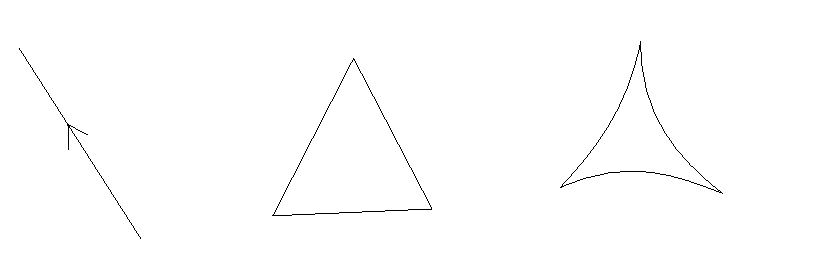
\includegraphics[width=0.8\textwidth]{img/boundary.pdf}
        \caption{Boundary Map}
        \label{fig:boundary}
    \end{figure}

    \(\sigma : \Delta^1 \to X\)

    \(\partial \sigma = \sigma(e_1) - \sigma(e_0) = c_{\sigma(e_1)}=c_{\sigma(e_0)}\), endpoint - starting point.
    
    \begin{lemma}
        \(\partial_{n+1} \circ \partial_n = 0\).

        \begin{center}
            \begin{tikzcd}
                S_{n+1} X \ar[r,"\partial_{n+1}"] \ar[rr, bend right, "0"] & S_n X \ar[r,"\partial_n"] & S_{n-1} X
            \end{tikzcd}
        \end{center}

        This is the reason for \(-\) signs.
    \end{lemma}

    Then, we have,

    \[
        \begin{matrix}
            \operatorname{im} \partial_{n+1} & \subset & \ker \partial_n & \subset & S_n X \\
            n \text{-boundaries} &  & n \text{-cycles} &  & n \text{-chains}  \\
        \end{matrix} 
    \]

    \begin{definition}
        [Singular Homology]

        \[
            H_n X = \frac{\ker \partial_n}{\operatorname{im} \partial_{n+1}} = \frac{\text{cycles}}{\text{boundaries}}
        \]
    \end{definition}

    \begin{proof}
        We prove the lemma: \(\partial_{n-1} \circ \partial_n = 0\).

        \[
            \partial_{n-1} (\partial_n \sigma)
        \]

        \[
            = \partial_{n-1} \left( \sum_{j} (-1)^{j} \sigma(t_0, \cdots , 0, \cdots , t_{n-1}) \right) 
        \]

        \[
            = \sum_{k < j} (-1)^k (-1)^j \sigma(t_0, \cdots , 0, \cdots , 0, \cdots , t_n) \, \text{\(0\) s in \(k\)'th and \(j\)'th slots}
        \]

        \[
            + \sum_{k > j} (-1)^{k-1} (-1)^j \sigma(t_0, \cdots , 0, \cdots , 0, \cdots , t_n) \, \text{\(0\) s in \(k\)'th and \(j\)'th slots}
        \]

        \[
            = 0
        \]
    \end{proof}

    \begin{remark}
        \begin{enumerate}[label=\arabic*)]
            \item \(H_n X\) is defined for any topological space \(X\) and \(n \geq 0\).
            
            \item \(X \cong Y \implies H_n X \cong H_n Y\).
            
            \item Big and Formula Construction.
            
            \item Unclear how to compute.
        \end{enumerate} 
    \end{remark}

    Answer to the question: What is \(H_n X\):

    \[
        H_{\ast} X = \left\{ H_0 X, H_1 X, H_2 X , \cdots  \right\} 
    \]

    is a graded abelian group. \(H_k X\) individually are abelian groups.

    \begin{lemma}[Lemma 1]
        \[
            H_n(pt) \cong \begin{dcases}
                \mathbb{Z}, &\text{ if } n = 0 ;\\
                0, &\text{ otherwise} .
            \end{dcases}
        \]
    \end{lemma}

    \begin{lemma}[Lemma 2]
        If \(X\) has path-components \(\{ X_\alpha \}_{\alpha \in I}\), then,

        \[
            H_n X = \bigoplus_{\alpha \in I} H_n (X_\alpha)
        \]
    \end{lemma}

    \begin{lemma}
        [Lemma 3]
        \begin{enumerate}[label=\alph*)]
            \item \( H_0 X \cong \bigoplus_{I} \mathbb{Z} = \mathbb{Z}^{\# \text{ of path component}}\)
            \item \(X\) is path-connected, then \(H_0 X \cong \mathbb{Z}\).
        \end{enumerate} 
    \end{lemma}

    Recall:

    \begin{definition}
        \(X\) is path-connected if \(\forall a,b\in X, \exists \gamma: [0,1] \to X\) such that \(\gamma(0)=a, \gamma(1)=b\) 
    \end{definition}

    \begin{definition}
        A maximal path-connected subset of \(X\) is path-component.
    \end{definition}

    \begin{corollary}
        Homology of rational numbers is isomorphic to the homology of integers:

        \[
            H_{\ast} \mathbb{Q} \cong H_{\ast} \mathbb{Z} = (\mathbb{Z}^{\infty}, 0, 0, \cdots)
        \]

        But \(\mathbb{Q} \not\cong \mathbb{Z}\).
    \end{corollary}

    \section*{Friday, 1/17/2025}
    
    Recall:

    \(H_n X = \frac{\ker (\partial_n)}{\operatorname{im} (\partial_{n+1})} = \frac{\text{cycles}}{\text{boundary}} \in \text{homology class}\).

    We are looking for two cycles that belong to the same homology class.

    So, we want cycles \(z_1 \neq z_2\) which are homologous so that \(z_1 - z_2\) is a boundary. This implies their homology classes are equal: \([z_1] = [z_2]\).

    % insert 0 cycle example

    % insert torus example

    \section*{Algebra}

    \begin{definition}
        [Chain Complex] A \underline{chain complex} \(C_\bullet\) is a sequence:
        
        \[
            C_{\ast} = \{ C_0, C_1, C_2, \cdots \}
        \]
        
        of abelian groups with \(\partial_n : C_n \to C_{n-1}\) such that \(\partial_n \circ \partial_{n+1} = 0\).

        It looks like the following:

        \begin{center}
            \begin{tikzcd}
                \cdots \ar[r] & C_3 \ar[r, "\partial_3"] & C_2 \ar[r,"\partial_2"] & C_1 \ar[r,"\partial_1"] & C_0
            \end{tikzcd}
        \end{center}

        so that the composition of any two consecutive maps is \(0\). By conventions, \(\partial_0 = 0: C_0 \to 0\).
    \end{definition}

    Then, \(C_\bullet = \{ C_{\ast}, \partial_{\ast} \}\).

    \begin{definition}
        [Homology]

        \[
            H_n C_\bullet = \frac{\ker \partial_n}{\operatorname{im} \partial_{n+1}} = \frac{Z_n}{B_n}
        \]

        Here, \(C_n = n\)-chain.
        
        \(Z_n = \ker \partial_n, n\)-cycles
        
        \(B_n = \operatorname{im} \partial_{n+1}, n\)-boundaries.

        eg. \(S_\bullet X = \{ S_{\ast} X, \partial_{\ast} \}\) is a singular chain complex of \(X\).
    \end{definition}

    L1:

    \[
        H_n \text{pt} = \begin{dcases}
            \mathbb{Z}, &\text{ if } n=0 ;\\
            0, &\text{ otherwise} .
        \end{dcases}
    \]

    \[
        H_{\ast} (\text{pt}) = \{ \mathbb{Z},0,0,\cdots \}
    \]

    \begin{proof}
        \(\forall n, \exists ! \sigma_n : \Delta^n \to \text{pt}\).

        Then, \(\partial_1 \sigma_1 = \sigma_1 \circ \delta_0 - \sigma_1 \circ \delta_1\).

        \(\delta_0(t_0) = (0,t_0), \delta_1(t_0) = (t_0, 1)\).

        Thus, \(\partial_1 \sigma_1 = \sigma_1 \circ \delta_0 - \sigma_1 \circ \delta_1=(1-1)\sigma_0 = 0\)
        
        \(\partial_2 \sigma_2 = \sigma_2 \circ \delta_0 - \sigma_2 \circ \delta_1 + \sigma_2 \circ \delta_2 = (1-1+1)\sigma_1 = \sigma_1\).

        \(\partial_n \sigma_n = \begin{dcases}
            0, &\text{ if } n \text{ odd} ;\\
            1, &\text{ if } n \text{ even}.
        \end{dcases}\) 

        \(S_{\ast} X:\)
        
        \begin{center}
            \begin{tikzcd}
                & & \ar[r] & \mathbb{Z}\sigma_2 \ar[r] & \mathbb{Z}\sigma_1 \ar[r] & \mathbb{Z}\sigma_0 \\

                & & & \sigma_2 \ar[r,mapsto] & \sigma_1 \ar[r,mapsto] & 0 \\
                \cong & \ar[r,"1"] & \mathbb{Z} \ar[r,"0"] & \mathbb{Z} \ar[r,"1"] & \mathbb{Z} \ar[r,"0"] & \mathbb{Z}
            \end{tikzcd}
        \end{center}

        \(H_0 \text{pt} = \mathbb{Z} / 00 = \mathbb{Z}\).

        \(H_1 \text{pt} = \mathbb{Z} / \mathbb{Z} = 0\) 

        \(H_2 \text{pt} = 0 / 0 = 0\).
    \end{proof}

    L2: If \(\{ X_\alpha \}_{\alpha \in I}\) are path components of \(X\) then,

    \[
        H_n X = \bigoplus_{I} H_n X_\alpha
    \]

    \begin{proof}
        \(\sigma: \Delta^n \to X \overset{\Delta^n \text{p.c.}}{\implies} \sigma(\Delta^n)\) p.c.

        \(\implies \exists ! \alpha\) such that \(\sigma(\Delta^n) \subset X_\alpha\).

        Also \((\sigma \circ \delta_j)(\Delta^{n-1}) \subset X_\alpha\)
        
        \(S_{\ast} X = \bigoplus_{I} S_{\ast} X_\alpha\) 
    \end{proof}

    Augmentation

    \(\varepsilon : S_0 X \to \mathbb{Z}\)

    \(\varepsilon (\sum_{i} n_i \sigma_i) \coloneqq \sum_{i} n_{i}\)
    
    \(\varepsilon  \circ \partial_1 (\sigma) = \varepsilon  (\sigma \circ \delta_0 - \sigma \circ \delta_1) = 1-1 = 0\)

    Thus \(\operatorname{im} \partial_1 \subset \ker \mathscr{E}\)

    Thus, \(\exists \overline{\varepsilon}: H_0 X \to \mathbb{Z}\)

    \(\overline{\varepsilon} \left[\sum_{i} n_i \sigma_i\right] = \varepsilon \left( \sum_{i} n_i \sigma_i \right) = \sum_{i} n_i \). 

    L3:

    \begin{enumerate}[label=\arabic*)]
        \item If \(X\) is path connected then,
        
        \[
            \overline{\varepsilon}: H_0 X \xrightarrow{\cong}\mathbb{Z}
        \]

        \item If \(\{ X_\alpha \}_{\alpha \in I}\) are path components of \(X\) then,
        
        \[
            H_0 X = \bigoplus_{I} H_0 X_\alpha = \mathbb{Z}^{\text{\# of p.c. of } X} 
        \]
    \end{enumerate}
    
    \begin{proof}
        \begin{enumerate}[label=\arabic*)]
            \item Need to show \(\ker \varepsilon \subset \operatorname{im} \partial_1\).
            
            Choose base point \(x_0 \in X\).

            Suppose \(\varepsilon \left( \sum_{i} n_i \sigma_i \right) = 0\).

            Choose path \(\gamma_i: \Delta^1 \to X\) such that \(\gamma_i(\underline{e}_1) = \sigma_i(\underline{e}_0), \gamma_0(e_0) = x_0\).
            
            \(\partial_1 \left( \sum_{i} n_i \gamma_i \right) = \sum_{i} n_i \sigma_i - \sum_{i} n_i \text{cons}_{X_0} = \sum_{i} n_i \sigma_i \) 
        \end{enumerate} 
    \end{proof}

    \section*{\(\Delta\)-complex (p.102-104 of Hatcher)}

    eg torus

    \begin{center}
        \begin{tikzpicture}
            \draw[->] (0,0) -- (2,0);
        \end{tikzpicture}
    \end{center}

    % insert torus picture

    \(1 =\) \# of vertices
    
    \(3 =\) \# of edges

    \(2 =\) \# of faces

    \(\Delta_2 T \to \Delta_1 T \to \Delta_0 T\) 

    \(\cong \mathbb{Z}^2 \to \mathbb{Z}^3 \to \mathbb{Z}^1\) 

    \section*{Wednesday, 1/22/2025}
    
    \begin{definition}
        [Simplex] Let \(v_0, \cdots , v_n \in \mathbb{R}^n\).

        \[
            [v_0, \cdots , v_n] = \left\{ \sum_{i} t_i v_i \mid \sum_{i} t_i = 1, 1 \leq t_i \leq 0 \right\}
        \]

        If \(v_0 - v_1, \cdots , v_0 - v_n\) are linearily independent, then \([v_0, \cdots , v_n]\) is a \underline{geometric} \underline{\(n\)-simplex}.
    \end{definition}

    If vertices are ordered,

    \[
        \sigma_{[v_0, \cdots , v_n]} : \Delta^n \to [v_0, \cdots , v_n]
    \]

    \[
        \sum_{i} t_i e_i \mapsto \sum_{i} t_i v_i
    \]

    Note that,

    \[
        \delta_n \sigma_{[v_0, \cdots , v_n]} \equiv  \sum_{j} (-1)^j \sigma_{[v_0, \cdots , \widehat{v_j}, \cdots , v_n]}
    \]

    \(\Delta^n\) breaks up into boundary and interior.

    \[
        \Delta^n = \partial \Delta^n \cup \mathring{\Delta^n}
    \]

    \[
        \partial \Delta^n = \left\{ \sum_{i} t_i e_i \mid \text{some } t_i = 0 \right\} 
    \]

    \[
        \mathring{\Delta^n} = \left\{ \sum_{i} t_i e_i \mid t_i\neq 0 \text{ for all } i \right\} 
    \]

    \begin{definition}
        A \(\Delta\)-complex is a space \(X\) with:

        \[
            \left\{ \sigma_\alpha : \Delta^n \to X \right\} \, \text{simplices} 
        \]

        such that:

        \begin{enumerate}[label=\roman*)]
            \item \(\eval{\sigma_\alpha}_{\mathring{\Delta^n}}\) is injective.
            
            \(\forall x\in X, \exists !\) s.t. \(x\in \sigma_\alpha(\mathring{\Delta^n})\). Images of interiors partition \(X\).

            \item \(\forall \alpha, \forall j, \exists \beta\) such that:
            
            \[
                \sigma_\alpha \circ \delta_j = \sigma_\beta
            \]

            Faces of simplices are simplices.

            \item \(A \subset X\) open \(\iff \forall \sigma_\alpha, \sigma_\alpha ^{-1} A\) is open in \(\Delta^n\). ``Weak Topolofy''.
        \end{enumerate} 


    \end{definition}

    Hatcher says, one way to look at this is by taking a quotient of a disjoint union. We can consider:

    \[
        \frac{\Delta^0 \sqcup \Delta^1 \sqcup \Delta^1 \sqcup \Delta^1 \sqcup \Delta^2 \sqcup \Delta^2}{\sim}
    \]

    \begin{definition}
        [Simplicial Chain Complex] \(\Delta_n X =\) free abelian group on \(n\)-simplices:

        \[
            \Delta_{n+1} X \xrightarrow{\partial_{n+1}} \Delta_n X \to \Delta_{n-1} X \to 
        \]

        Subcompplex \(\Delta_{\ast} X \subset S_{\ast} X\) 

        \begin{center}
            \begin{tikzcd}
                \Delta_n X \ar[r,"\partial"] \ar[d, hook] & \Delta_{n-1} X \ar[d, hook] \\ S_n X \ar[r,"\partial"] & S_{n-1} X
            \end{tikzcd}
        \end{center}

        The diagram commutes.

        Simplicial Homology:

        \[
            H_{\ast} ^\Delta X \coloneqq H_{\ast} (\Delta_{\ast} X)
        \]

        \[
            H_{\ast}^\Delta X \xrightarrow{\cong} H_{\ast} X
        \]
        
    \end{definition}

    Consider the \(2\)-torus with ``ordered'' vertices:

    % insert picture

    % insert picture

    \[
        \partial U = b-c+a
    \]

    \[
        \partial L = a-c+b
    \]

    \[
        \partial a = 0v, \partial b = 0v, \partial c = 0v
    \]

    \[
        \Delta_2 T \to \Delta_1 T \to \Delta_0 T \to 0
    \]

    Then, \(\Delta_2 T\) has basis \(\mathbb{Z} U \oplus \mathbb{Z} L\)

    \(\Delta_1 T\) has basis \(\mathbb{Z} a \oplus \mathbb{Z} b \oplus \mathbb{Z} c\)
    
    \(\Delta_0 T\) has basis \(\mathbb{Z}v\)

    Now, \(H_0^\Delta T = \frac{\mathbb{Z} v}{0} \cong \mathbb{Z}\) 

    \(H_2^\Delta T = \frac{\mathbb{Z}(U-L)}{0}\cong \mathbb{Z}\).

    We only have \(U-L\) since \(\partial(n_1 U + n_2 L) = 0 \implies n_1(b-c+a) + n_2(a-c+b) = 0 \implies n_1 = -n_2\)

    \(H_1^\Delta T = \frac{\mathbb{Z}(a,b,c)}{\mathbb{Z}(a-c+b)} = \frac{\mathbb{Z}(a,b,a-c+b)}{\mathbb{Z}(a-c+b)} \cong \mathbb{Z}^2\).

    We can have a basis for homology since they are free abelian.

    Basis for \(H_0^\Delta T\) is \([v]\)
    
    Basis for \(H_1^\Delta T\) is \([a],[b]\).
    
    Basis of \(H_2^\Delta T\) is \([U-L]\).

    Matrix POV on \(H_{\ast}^\Delta T\)

    \[
        \Delta_\cdot \cong \mathbb{Z}^2 \xrightarrow{\begin{bmatrix}
            1 & 1 \\
            1 & 1 \\
            -1 & -1
        \end{bmatrix} } \mathbb{Z}^3 \xrightarrow{\begin{bmatrix}
            0 & 0 & 0
        \end{bmatrix}} \mathbb{Z}
    \]

    Integral row and column operations:

    \begin{itemize}
        \item Switch two rows (or columns)
        \item Add multiples of a row (or column) to another row (or column)
        \item Multiply row (or column) by \(\pm 1\) 
    \end{itemize} 

    These correspond to basis changes in the domain and codomain.

    If matries \(A\) and \(B\) are equivalent \((A \sim B)\) it implies:

    \[
        \ker A \cong \ker B
    \]

    \[
        \operatorname{coker}  A \cong \operatorname{coker} B
    \]

    Every integral matrix is equivalent to:

    \[
        \begin{bmatrix}
            d_1 &  &  &  \\
             & d_2 &  &  \\
             &  & \ddots &  \\
             &  &  & d_n \\
        \end{bmatrix} 
    \]

    With \(d_1 \mid d_2 \mid d_3 \mid \cdots\) 

    It is a smith normal form.

    We have:

    \[
        \begin{bmatrix}
            1 & 1 \\
            1 & 1 \\
            -1 & -1 \\
        \end{bmatrix} \sim \begin{bmatrix}
            1 & 0 \\
            1 & 0 \\
            -1 & 0 \\
        \end{bmatrix} \sim \begin{bmatrix}
            1 & 0 \\
            0 & 0 \\
            0 & 0 \\
        \end{bmatrix} 
    \]

    This is \(\partial_2\).

    \(H_2^\Delta T \cong \mathbb{Z}\) 

    \(\operatorname{im} \partial_2 \cong \mathbb{Z}\) and summand of \(\Delta_1 T\)

    \(H_1^\Delta T \cong \frac{\mathbb{Z}^3}{\mathbb{Z} \times 0 \times 0} \cong \mathbb{Z}^2\) 

    Exercise: compute kernel and cokernel of: \(\begin{bmatrix}
        9 & 3 \\
        4 & 2 \\
    \end{bmatrix} \) 

    \(\begin{bmatrix}
        9 & 3 \\
        4 & 2 \\
    \end{bmatrix} \sim \begin{bmatrix}
        5 & 1 \\
        4 & 2 \\
    \end{bmatrix} \sim \begin{bmatrix}
        5 & 1 \\
        -1 & 1 \\
    \end{bmatrix} \sim \begin{bmatrix}
        6 & 0 \\
        -1 & 1 \\
    \end{bmatrix} \sim \begin{bmatrix}
        6 & 0 \\
        0 & 1 \\
    \end{bmatrix} \sim \begin{bmatrix}
        1 & 0 \\
        0 & 6 \\
    \end{bmatrix} \) 

    Thus, \(\ker = 0, \operatorname{coker} = \mathbb{Z} / 6\mathbb{Z}\).

    \section*{Friday, 1/24/2025}
    
    Goal: if there is continuous \(f: X \to Y\) then we have homomorphism \(f_{\ast} : H_{\ast} X \to H_{\ast} Y\).
    
    We think of them in terms of Category Theory.

    Setup:

    Category \(\mathcal{C}\).

    Collection of objects \(\operatorname{Ob} \mathcal{C}\).

    \(\forall X, Y \in \operatorname{Ob} \mathcal{C}\) we have a collection of morphisms \(\mathcal{C}(X,Y)\).

    \(\forall X,Y,Z \in \operatorname{Ob} \mathcal{C}\) we have composition law:

    \[
        \mathcal{C}(X,Y) \times \mathcal{C}(Y,Z) \to \mathcal{C}(X,Z)
    \]

    \[
        (g,f) \mapsto f \circ g
    \]

    Also, \(\forall X\in \operatorname{Ob} \mathcal{C}, \exists \operatorname{id}_{X} \in \mathcal{C}(X,X)\).

    We also have associative law:

    \[
        (f \circ g) \circ h = f \circ (g \circ h)
    \]

    \(\forall f\in \mathcal{C}(X,Y), f = \operatorname{id}_{Y} \circ f = f \circ \operatorname{id}_{X}\).

    For \(f\in \mathcal{C}(X,Y)\) we can also write it as \(f: X \to Y\) or \(X \xrightarrow{f} Y\).

    We sometimes call them `arrows' instead of `morphisms' to avoid thinking of them as functions.

    \begin{center}
        \begin{tikzcd}
            X \ar[r,"g"] \ar[rr, bend right, "f\circ g"'] & Y \ar[r,"f"] & Z
        \end{tikzcd}
    \end{center}

    \begin{definition}
        \(f: X \to Y\) is an \underline{isomorphism} if \(\exists g: Y \to X\) such that:

        \[
            f \circ g = \operatorname{id}_{Y}, g \circ f = \operatorname{id}_{X} 
        \]

        We write it as \(X \cong Y\) and say \(X\) and \(Y\) are \underline{isomorphic}.
    \end{definition}

    Example of Categories:

    \(\operatorname{Set}\) is (sets, functions).

    \(\operatorname{Top}\) is (topological spaces, continuous functions)

    \(\operatorname{Ab}\) is (abelian groups, homomorphisms)

    Morphisms need not be functions!!

    A group can be viewed as a category with one object. Elements of the group is the set of morphisms, and all morphisms are invertible.

    Suppose \(G = \{ 1,T \}\) of order \(2\). Then, we have:

    \begin{center}
        \begin{tikzcd}
            T \ar[loop left, "T"] \ar[loop right, "\operatorname{id}"]
        \end{tikzcd}
    \end{center}

    Where \(T \circ T = \operatorname{id}\) 

    We let \(\operatorname{Ch}\) be the category of \underline{chain complexes}.

    The objects will be chain complexes. What are the morphisms?

    Recall that Chain complexes are \(C_\bullet = (C_{\ast} , \partial_{\ast})\) where:

    \begin{center}
        \begin{tikzcd}
            \, \ar[r] & C_{n+1} \ar[r,"\partial_{n+1}"] & C_n \ar[r,"\partial_n"] & C_{n-1} \ar[r] & \,
        \end{tikzcd}
    \end{center}

    Where \(\partial_{n+1} \circ \partial_n = 0\).
    
    Morphisms are given by \underline{chain maps}.

    \begin{definition}
        [Chain map] \(f_\bullet: C_\bullet \to C_\bullet^{\prime}\) is a sequence of homomorphisms \(f_n : C_n \to C_n^{\prime}\) such that:

        \[
            f_{n-1} \circ \partial_n = \partial_n^{\prime} \circ f_n
        \]

        For all \(n\).
    \end{definition}

    We have the following commutative diagram:

    \begin{center}
        \begin{tikzcd}
            \, \ar[r] & C_{n+1} \ar[d] \ar[r] & C_n \ar[d] \ar[r] & C_{n-1} \ar[d] \ar[r] & \, \\
            \, \ar[r] & C_{n+1}' \ar[r] & C_n' \ar[r] & C_{n-1}' \ar[r] & \,
        \end{tikzcd}
    \end{center}

    For example, if we have \(f: X \to Y\) we have the chain map:

    \[
        f_\# = S_\bullet f : S_\bullet X \to S_\bullet Y
    \]

    Given by:

    \[
        (S_{\bullet} f) \left( \sum_{i} n_i \sigma_i \right) \coloneqq \sum_{i} n_i (f \circ \sigma_i)
    \]

    % insert picture

    This gives us:

    \begin{center}
        \begin{tikzcd}
            S_n X \ar[r,"\partial_n"] \ar[d, "S_n f"] & S_{n-1} X \ar[d] \\ S_n Y \ar[r,"\partial_n"] & S_{n-1} Y
        \end{tikzcd}
    \end{center}

    \begin{lemma}
        A chain map \(f_\bullet: C_\bullet \to C_\bullet^{\prime} \) induces \(f_{\ast} = H_n(f_\bullet) : H_n C_\bullet \to H_n C_\bullet^{\prime}\) given by \([x] \mapsto [f_n x]\)  
    \end{lemma}

    \begin{remark}
        elements in \(\frac{\ker \partial_n}{\operatorname{im} \partial_{n+1}}\) can be \([x]\) [equivalence classes] or \(x + \operatorname{im} \partial_{n+1}\) [cosets]. We use equivalence classes:

        \(x \sim x^{\prime} \iff x - x^{\prime} \in \operatorname{im} \partial\) 
    \end{remark}

    \begin{proof}
        \(f_n(\text{cycles}) \subset \text{cycles}\).
        
        \(f_n(\text{boundaries}) \subset \text{boundaries}\).
        
        Recall that cycle is \(\ker \partial_n\).

        Consider a cycle \(X\). Then, \(\partial X = 0 \implies f(\partial x) = 0 \implies \partial ^{\prime} f(x) = 0 \implies f(x) \in \ker \partial ^{\prime}\).

        Boundary is \(\operatorname{im} \partial_{n+1}\).

        \(f(\partial y) = \partial ^{\prime} f(y) \in \operatorname{im} \partial_{n+1}^{\prime}\).

        Thus we have:
        
        \[
            \ker \partial_n \to \ker \partial_n^{\prime} \to \frac{\ker \partial_n^{\prime}}{\operatorname{im} \partial_{n+1}^{\prime}}
        \]

        This induces,

        \[
            \frac{\ker \partial_n}{\operatorname{im} \partial_{n+1}} \to \frac{\ker \partial_n^{\prime}}{\operatorname{im} \partial_{n+1}^{\prime}}
        \]

    \end{proof}

    Now we move on to functors. Functors are an analogy of functions on Categories.

    Consider two categories \(\mathcal{C}\) and \(\mathcal{D}\). We want to define a functor between them.

    \begin{definition}
        A functor \(F: \mathcal{C} \to \mathcal{D}\) will be an `assignment' of objects and morphisms.
        
        We have \(F: \operatorname{Ob} \mathcal{C} \to \operatorname{Ob} \mathcal{D}\).
        
        \(\forall X,Y \in \operatorname{Ob} \mathcal{C}\) we have:

        \[
            F: \mathcal{C}(X,Y) \to \mathcal{D}(F(X),F(Y))
        \]

        Then, \(F(f \circ g) = F(f) \circ F(g)\).

        \(F(\operatorname{id}_{X}) = \operatorname{id}_{F(X)}\) 
    \end{definition}

    So we can \(F\) a whole category:

    \[
        X \xrightarrow{f} Y
    \]

    \[
        F(X) \xrightarrow{F(f)} F(Y)
    \]

    We have the \underline{singular} functor taking topological spaces to chain complexes. We also have functor taking chain complexes to abelian groups.

    \[
        \operatorname{Top} \xrightarrow{S_\bullet} \operatorname{Ch} \xrightarrow{H_n} \operatorname{Ab} 
    \]

    We also have forgetful functor which forgets:

    \[
        \operatorname{Ab} \to \operatorname{Set} 
    \]

    \[
        \operatorname{Ab} \to \operatorname{Group} 
    \]

    We have the category \(\operatorname{Gr}\) of graded abelian groups.

    \(\operatorname{Gr}\) has objects \(A_{\ast} = \{ A_0, A_1, A_2, \cdots \} \) set of abelian groups, and morphisms \(A_{\ast} \xrightarrow{f_0} B_{\ast}\).
    
    Then we can write:

    \begin{center}
        \begin{tikzcd}
            \operatorname{Top} \ar[r,"S_\bullet"] \ar[rrr, bend right, "H_n"] & \operatorname{Ch} \ar[r,"H_{\ast}"] & \operatorname{Gr} \ar[r,"H_n"] & \operatorname{Ab}
        \end{tikzcd}
    \end{center}

    \begin{lemma}
        Consider a functor \(F: \mathcal{C} \to \mathcal{D}\). Then, \(X \cong Y \implies F(X) \cong F(Y)\).
    \end{lemma}

    Corollary: \(X \cong Y\) (homeomorphic) implies \(H_n X \cong H_n Y\) 

    \begin{proof}
        \(X\cong Y\) implies we have \(f,g\) so that \(f(X)=Y, g(Y) = X\) so that \(f \circ g = \operatorname{id}_{Y}, g \circ f = \operatorname{id}_{X}\).
        
        Then, \(F(f) \circ F(g) = F(f \circ g) = F(\operatorname{id}_{Y}) = \operatorname{id}_{F(Y)}\). Similar for \(g \circ f\). So, \(F(f)\) and \(F(g)\) are isomorphisms and thus \(F(X)\) and \(F(Y)\) are isomorphic. 
    \end{proof}

    \section*{Monday, 1/27/2025}
    
    \section*{Homotopy Invariance of Homology}

    \begin{definition}
        [Homotopy] \(H: X \times I \to Y\, I = [0,1]\).

        Homotpy is a `path' of map \(H_t: X \to Y\) where \(t\in [0,1]\) is `time'. \(H_t(x) = H(x,t)\).
    \end{definition}

    % insert picture

    \begin{definition}
        \(f,g : X \to Y\) are \underline{homotopic} if there exists \(H: X \times I \to Y\) such that \(H_0 = f, H_1 = g\).
    \end{definition}

    If they're homotopic we write \(f\simeq g\).

    \begin{theorem}
        [Homotopy Theorem]

        \[
            f \simeq g \implies H_{\ast} f = H_{\ast} g: H_{\ast} X \to H_{\ast} Y
        \]

        \[
            f_{\ast} = g_{\ast} 
        \]
    \end{theorem}

    Fact/Exercise: \(\simeq\) is a equivalence relation on \(\operatorname{TOP}(X,Y)\) 

    \([X,Y] = \operatorname{TOP}(X,Y) / \simeq =\) homotopy classes of map \(X \to Y\).

    Suppose for \(X,Y\), \(X \xleftrightarrow[g]{f} Y\) we have \(f \circ g \simeq \operatorname{id}_X,X \cong H_{\ast} Y\).
    
    For example, \(\mathbb{R}^2 - 0 \simeq S^1\). by \(x \xmapsto{f} \frac{x}{\vert x \vert}\) and \(g = \text{inclusion}\).

    Straight line homotopy \(tx + (1-t) \frac{x}{\vert x \vert}\)

    \begin{definition}
        \(X\) \underline{contractible} if \(X \simeq pt\).

        eg \(\mathbb{R}^2 \simeq \ast\) 
    \end{definition}

    % insert picture

    \begin{definition}
        Homotopy Category \(\operatorname{hTOP}\).

        \underline{Objects}: Topological Spaces [\underline{NOT} HOMOTOPY EQUIVALENCE CLASSES]

        \underline{Morphisms}: \(\operatorname{hTOP}(X,Y) = [X,Y]\). [These are Equivalence Classes]
        
        \underline{Exercise}: Composition is well defined. So, \(f \simeq f^{\prime} , g \simeq g^{\prime} \implies f \circ g \simeq f
        \circ g^{\prime}\). Then, \([f] \circ [g] \coloneqq [f \circ g]\) 
    \end{definition}

    \subsection*{Isomorphisms in hTOP}

    \(X,Y\) Isomorphic in \(\operatorname{hTOP} \iff X \simeq Y\) [homotopy equivalence].

    So, homotopy theorem says homology factors through homotopy:

    \begin{center}
        \begin{tikzcd}
            \operatorname{hTop}\ar[r,"H_\ast"] & \operatorname{Gr} \\ \operatorname{TOP} \ar[u] \ar[ur, "H_\ast"']
        \end{tikzcd}
    \end{center}

    Thus, \(X \simeq Y \iff H_{\ast} X \implies H_{\ast} Y\) is really just a consequence of homotopy theorem.

    \begin{definition}
        \(A \subset X\), then \(A \) is a \underline{deformation retract} of \(X\) `if we can deform all of \(X\) into \(A\)'. Formally,

        if \(\exists H: X \times I \to X\) such that:
        
        \(\forall x\in X, H(x,0)=x, H(x,1)\in A\) and \(H(a,1)=a \forall a\in A\).

        Suppose \(A \simeq X\), \(A \xhookrightarrow{i} X, A \xleftarrow{H_1} X\).

        \(\operatorname{id}_{A} = H_1 \circ i, \operatorname{id}_{X} \underset{H}{\simeq} i \circ H_1\)

        eg M\"obius strip \((X)\) is homotopy equivalent to the cure circle \(A\).

        % insert picture

        \begin{definition}
            \(X \subset \mathbb{R}^n\) is start shaped at \(p_0 \in X\) if \(\forall p\in X, \overline{pp_0} \subset X\).
        \end{definition}

        % insert picture

        convex \(\implies\) star-shaped \(\implies\) contractable (by the straight line homotopy)

        We can take \((1-t)p_0 + ^{\top}  = H(p,t)\).

        eg the \(n\)-simplex \(\Delta^n\) and the prism \(\Delta^n \times I\) are star-shaped.

    \end{definition}

    \begin{theorem}
        \(X\) start shaped \(\implies H_{\ast} (X) = \mathbb{Z}\) or \(0\).
    \end{theorem}

    \begin{corollary}
        \(H_{\ast} (\Delta^n) \cong H_{\ast} (pt)\)

        \(H_{\ast} (\Delta^n \times I) \cong H_{\ast} (p t)\).
    \end{corollary}

    \begin{proof}
        Wlog \(\sigma : \Delta^n \to X\).

        Syspension \(s \sigma : \Delta^{n=1} \to X\):

        \[
            s \sigma(t_0, \cdots , t_{n+1}) = \begin{dcases}
                (1-t_0) \sigma \left( \frac{t_1}{1-t_0}, \cdots , \frac{t_{n+1}}{1-t_0} \right), &\text{ if }  t_0 \neq 1 ;\\
                0, &\text{ if } t_0 = 1 .
            \end{dcases}
        \]

        % insert picture

        We will show that if \(z\) is a \(n\)-cycle with \(n > 0\) then \(z = \partial (s z) \implies z\) is a boundary.

        Define: \(0\)th face of \(s \sigma\) is \(\sigma\).

        \((s \sigma) \circ \delta_0 = \sigma\)

        \((s \sigma) \circ \delta_{j+1} = s(\sigma \circ \delta_j) \implies s \partial + \partial s = \operatorname{id}_{S_n X} \, \forall n > 0\).

        Thus if \(z \in S_n X\) then ,

        \(s \partial z + \partial s z = z \implies \partial(sz) = z \implies z\) is a boundary.
    \end{proof}

    \subsection*{Algebra}

    \begin{definition}
        Chain map \(f_\bullet, g_\bullet: C_\bullet \to C_{\bullet}^{\prime}\) are \underline{chian} \underline{homotopic} if \(\exists\) homomorphisms \(h_n : C_n \to C_{n+1}
    ^{\prime}\)  `degree one' such that:

    \[
        \partial ^{\prime} h + h_{n-1} \partial _n = f_n - g_n
    \]

    \begin{center}
        \begin{tikzcd}
            C_{n+1} \ar[r] & C_n \ar[ld,"h"] \ar[d, "f\,g"] \ar[r] & C_{n-1} \ar[ld, "h"] \\ C_{n+1}^\prime \ar[r] & C_n^\prime \ar[r] & C_{n-1}^\prime
        \end{tikzcd}
    \end{center}
    \end{definition}

\end{document} 